%\VignetteIndexEntry{MeSH.db}
\documentclass[11pt]{article}
\usepackage{Sweave}
\usepackage{amsmath}
\usepackage{hyperref}
\usepackage{cite}
\usepackage{Sweave}

\usepackage[numbers]{natbib}
\usepackage{amsmath}
\usepackage{amssymb}
\Sconcordance{concordance:MeSH.db.tex:MeSH.db.Rnw:%
1 221 1 4 0 1 3 5 1 17 0 1 3 6 1 7 0 1 3 5 1 7 0 1 3 6 1 14 0 1 4 5 1 9 %
0 1 4 5 1 8 0 1 3 10 1 7 0 1 3 5 1 7 0 1 3 6 1 10 0 1 5 8 1 5 0 1 4 2 1 %
9 0 1 3 6 1 45 0 1 4 4 1 10 0 1 5 5 1 8 0 1 3 4 1 50 0 1 5 5 1 18 0 1 5 %
4 1 16 0 1 3 10 1 23 0 1 3 51 1}

\usepackage{url}
\usepackage[utf8]{inputenc}

\setlength{\textheight}{8.5in}
\setlength{\textwidth}{6in}
\setlength{\topmargin}{-0.25in}
\setlength{\oddsidemargin}{0.25in}
\setlength{\evensidemargin}{0.25in}
\newcommand{\Rpackage}[1]{{\textit{#1}}}

\usepackage{Sweave}
\begin{document}





\title{\bf How to use the MeSH.db Package}
\author{Koki Tsuyuzaki$^1$, Itoshi Nikaido$^2$$^,$$^3$ and Gota Morota$^4$.}
\maketitle
\begin{center}
\noindent
$^1$Department of Medical and Life Science, Tokyo University of Science.\\
\noindent
$^2$Functional Genomics Unit, RIKEN Center for Developmental Biology.\\
\noindent
$^3$Laboratory for Systems Biology, RIKEN Center for Developmental Biology.\\
\noindent
$^4$Department of Animal Sciences, University of Wisconsin-Madison.\\
\end{center}

\begin{center}
{\tt k.t.the-answer@hotmail.co.jp}
\end{center}
\tableofcontents

%%%%%%%%%%%%%%%%%%%%%%%%%%%%%%%%%%%%%%%%%%%%%%%%%%%%%%%%%%%%%%%%%%
%\clearpage
\newpage
\section{Introduction}
This document provides the way to use \Rpackage{MeSH.db} package. MeSH (Medical Subject Headings) is the NLM controlled vocabulary used to manually index articles for MEDLINE/Pubmed \cite{Nelson2004}. 

%%%%%%%%%%%%%%%%%%%%%%%%%%%%%%%%%%%%%%%%%%%%%%%%%%%%%%%%%%%%%%%%%%
\begin{figure}[ht]
\centering
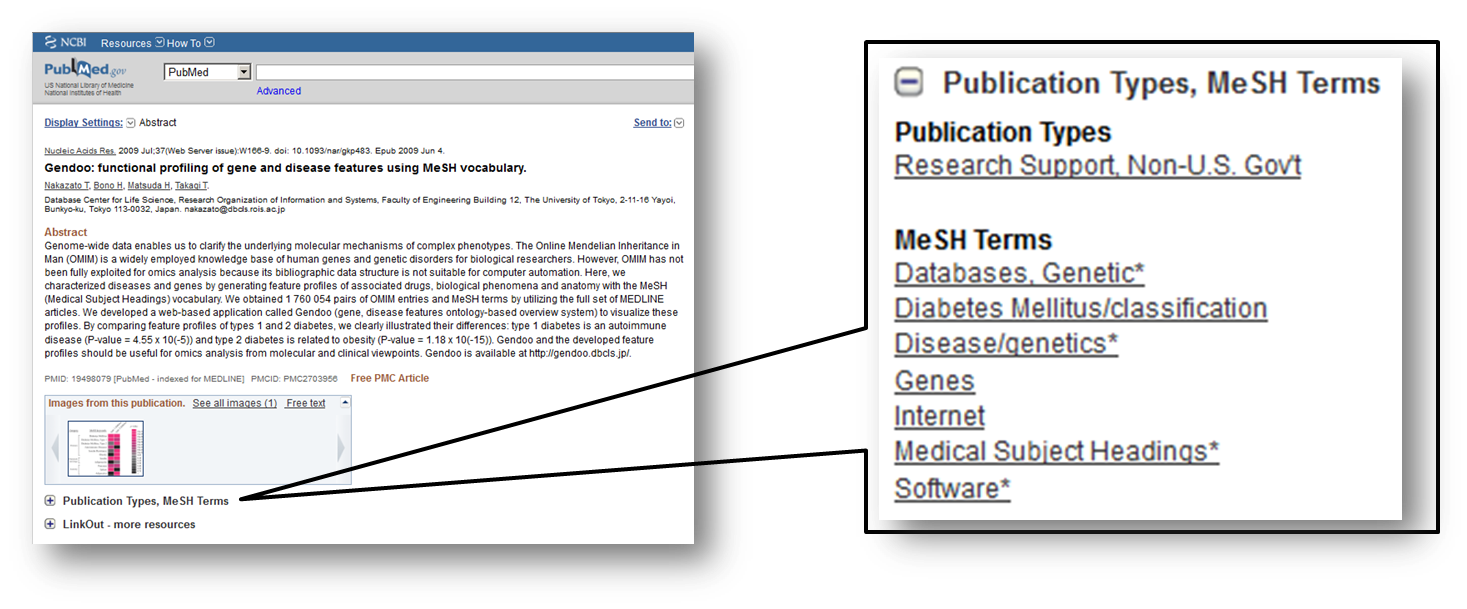
\includegraphics[width=\linewidth]{fig1.png}
\caption{MeSH Term}
\label{fig1}
\end{figure}
%%%%%%%%%%%%%%%%%%%%%%%%%%%%%%%%%%%%%%%%%%%%%%%%%%%%%%%%%%%%%%%%%%

The amount of vocabulary in MeSH is about twice as large as that of GO (Gene Ontology)\cite{Ashburner2000} and its category is also wider. Therefore MeSH is expected to be much detailed and exhaustive gene annotation tool. Some softwares or databases using MeSH are now proposed \cite{Nakazato2007,Nakazato2009,Saurin2010,Sartor2012}.\\
\Rpackage{MeSH.db} is a free R package for handling MeSH in R. Its data are retrieved from NLM ftp site (\url{http://www.nlm.nih.gov/mesh/filelist.html}). MeSH in 2013 has 19 hierarchies and MeSH.db provides 16 of them, which are actually assigned to some MeSH Terms. Each category is expressed as single capital alphabet defined by NLM as abbreviations.

\begin{center}
  \begin{table}[htbp]
    \begin{tabular}{|c|l|}\hline
      Abbreviation & Category \\ \hline \hline
      A & Anatomy \\ \hline
      B & Organisms \\ \hline
      C & Diseases \\ \hline
      D & Chemicals and Drugs \\ \hline
      E & Analytical, Diagnostic and Therapeutic Techniques and Equipment \\ \hline
      F & Psychiatry and Psychology \\ \hline
      G & Phenomena and Processes \\ \hline
      H & Disciplines and Occupations \\ \hline
      I & Anthropology, Education, Sociology and Social Phenomena \\ \hline
      J & Technology and Food and Beverages \\ \hline
      K & Humanities \\ \hline
      L & Information Science \\ \hline
      M & Persons \\ \hline
      N & Health Care \\ \hline
      V & Publication Type \\ \hline
      Z & Geographical Locations \\ \hline
\end{tabular}
  \end{table}
\end{center}

\newpage
MeSH has hierarchical structures like GO. \Rpackage{MeSH.db} provides its Ancestor-Offspring Relationships (AOR) and Parent-Child Relationships (PCR) as corresponding table (dataframe). Data of PCR and AOR are also used for calculating the conditional probability in enrichment analysis (\Rpackage{meshr} package).
%%%%%%%%%%%%%%%%%%%%%%%%%%%%%%%%%%%%%%%%%%%%%%%%%%%%%%%%%%%%%%%%%%
%\clearpage
\newpage
\section{Getting started}
To load the \Rpackage{MeSH.db} package, just type library(MeSH.db). 5 methods and 36 data are provided by \Rpackage{MeSH.db}.
%%%%%%%%%%%%%%%%%%%%%%%%%%%%%%%%%%%%%%%%%%%%%%%%%%%%%%%%%%%%%%%%%%
%\clearpage
\section{Methods}
Following 5 methods are provided by \Rpackage{MeSH.db}.
\begin{center}
  \begin{table}[htbp]
    \begin{tabular*}{150mm}{@{\extracolsep{\fill}}|c|l|}\hline
      MeSH & Function for retrieval of the summary of all object in MeSH.db \\ \hline
      MeSH\_dbconn & Function for retrieval of the connection of .sqlite database\\ \hline
      MeSH\_dbfile & Function for retrieval of the directory of .sqlite file \\ \hline
      MeSH\_dbschema & Function for retrieval of the schema of .sqlite database \\ \hline
      MeSH\_dbInfo & Function for retrieval of the information of .sqlite database \\ \hline
\end{tabular*}
  \end{table}
\end{center}
%%%%%%%%%%%%%%%%%%%%%%%%%%%%%%%%%%%%%%%%%%%%%%%%%%%%%%%%%%%%%%%%%%
%\clearpage
\section{Data}
Following 36 data are provided by \Rpackage{MeSH.db}.
\\
\begin{center}
  \begin{table}[htbp]
    \begin{tabular*}{150mm}{@{\extracolsep{\fill}}|p{40mm}|p{100mm}|}\hline
      MeSHMAPCOUNTS & The number of row of all data \\ \hline
      MeSHTERM & MeSH Term\\ \hline
      MeSHSYNONYM & The synonym of MeSH Term \\ \hline
      MeSHQUALIFIER & Substantial Information of MeSH Term \\ \hline \hline
      MeSHAAOR & Ancestor-Offspring Relationships in A category \\ \hline
      MeSHBAOR & Ancestor-Offspring Relationships in B category \\ \hline
      MeSHCAOR & Ancestor-Offspring Relationships in C category \\ \hline
      MeSHDAOR & Ancestor-Offspring Relationships in D category \\ \hline
      MeSHEAOR & Ancestor-Offspring Relationships in E category \\ \hline
      MeSHFAOR & Ancestor-Offspring Relationships in F category \\ \hline
      MeSHGAOR & Ancestor-Offspring Relationships in G category \\ \hline
      MeSHHAOR & Ancestor-Offspring Relationships in H category \\ \hline
      MeSHIAOR & Ancestor-Offspring Relationships in I category \\ \hline
      MeSHJAOR & Ancestor-Offspring Relationships in J category \\ \hline
      MeSHKAOR & Ancestor-Offspring Relationships in K category \\ \hline
      MeSHLAOR & Ancestor-Offspring Relationships in L category \\ \hline
      MeSHMAOR & Ancestor-Offspring Relationships in M category \\ \hline
      MeSHNAOR & Ancestor-Offspring Relationships in N category \\ \hline
      MeSHVAOR & Ancestor-Offspring Relationships in V category \\ \hline
      MeSHZAOR & Ancestor-Offspring Relationships in Z category \\ \hline \hline
      MeSHAPCR & Parent-Child Relationships in A category \\ \hline
      MeSHBPCR & Parent-Child Relationships in B category \\ \hline
      MeSHCPCR & Parent-Child Relationships in C category \\ \hline
      MeSHDPCR & Parent-Child Relationships in D category \\ \hline
      MeSHEPCR & Parent-Child Relationships in E category \\ \hline
      MeSHFPCR & Parent-Child Relationships in F category \\ \hline
      MeSHGPCR & Parent-Child Relationships in G category \\ \hline
      MeSHHPCR & Parent-Child Relationships in H category \\ \hline
      MeSHIPCR & Parent-Child Relationships in I category \\ \hline
      MeSHJPCR & Parent-Child Relationships in J category \\ \hline
      MeSHKPCR & Parent-Child Relationships in K category \\ \hline
      MeSHLPCR & Parent-Child Relationships in L category \\ \hline
      MeSHMPCR & Parent-Child Relationships in M category \\ \hline
      MeSHNPCR & Parent-Child Relationships in N category \\ \hline
      MeSHVPCR & Parent-Child Relationships in V category \\ \hline
      MeSHZPCR & Parent-Child Relationships in Z category \\ \hline
    \end{tabular*}
  \end{table}
\end{center}

\newpage
In \Rpackage{MeSH.db}, all data are extracted by 4 functions defined by \Rpackage{AnnotationForge}; $\bf{keytypes}$, $\bf{cols}$, $\bf{keys}$ and $\bf{select}$. keys function has 1 parameter (keytype) and select function also has 3 parameters (keys, cols and keytype). cols is the columns which you can retrieved by select and keytype is the columns which you can specify as the parameter in keys and select functions.
\begin{center}
  \begin{table}[htbp]
    \begin{tabular*}{160mm}{@{\extracolsep{\fill}}|p{35mm}|p{55mm}|p{55mm}|} \hline
      Object Name & cols & keytype \\ \hline \hline
      MeSHMAPCOUNTS & MAPNAME, COUNT & MAPNAME \\ \hline
      MeSHTERM & \shortstack{MESHID, MESHTERM,\\ CATEGORY} & \shortstack{MESHID, MESHTERM,\\ CATEGORY} \\ \hline
      MeSHSYNONYM & MESHID, MESHSYNONYM & MESHID \\ \hline
      MeSHQUALIFIER & \shortstack{QUALIFIERID, SUBHEADING,\\ MESHID} & QUALIFIERID, MESHID \\ \hline \hline
      MeSHAAOR & \shortstack{ANCESTERMESHID,\\ OFFSPRINGMESHID} & \shortstack{ANCESTERMESHID,\\ OFFSPRINGMESHID} \\ \hline
     MeSHBAOR & \shortstack{ANCESTERMESHID,\\ OFFSPRINGMESHID} & \shortstack{ANCESTERMESHID,\\ OFFSPRINGMESHID} \\ \hline
     MeSHCAOR & \shortstack{ANCESTERMESHID,\\ OFFSPRINGMESHID} & \shortstack{ANCESTERMESHID,\\ OFFSPRINGMESHID} \\ \hline
     MeSHDAOR & \shortstack{ANCESTERMESHID,\\ OFFSPRINGMESHID} & \shortstack{ANCESTERMESHID,\\ OFFSPRINGMESHID} \\ \hline
     MeSHEAOR & \shortstack{ANCESTERMESHID,\\ OFFSPRINGMESHID} & \shortstack{ANCESTERMESHID,\\ OFFSPRINGMESHID} \\ \hline
     MeSHFAOR & \shortstack{ANCESTERMESHID,\\ OFFSPRINGMESHID} & \shortstack{ANCESTERMESHID,\\ OFFSPRINGMESHID} \\ \hline
     MeSHGAOR & \shortstack{ANCESTERMESHID,\\ OFFSPRINGMESHID} & \shortstack{ANCESTERMESHID,\\ OFFSPRINGMESHID} \\ \hline
     MeSHHAOR & \shortstack{ANCESTERMESHID,\\ OFFSPRINGMESHID} & \shortstack{ANCESTERMESHID,\\ OFFSPRINGMESHID} \\ \hline
     MeSHIAOR & \shortstack{ANCESTERMESHID,\\ OFFSPRINGMESHID} & \shortstack{ANCESTERMESHID,\\ OFFSPRINGMESHID} \\ \hline
     MeSHJAOR & \shortstack{ANCESTERMESHID,\\ OFFSPRINGMESHID} & \shortstack{ANCESTERMESHID,\\ OFFSPRINGMESHID} \\ \hline
     MeSHKAOR & \shortstack{ANCESTERMESHID,\\ OFFSPRINGMESHID} & \shortstack{ANCESTERMESHID,\\ OFFSPRINGMESHID} \\ \hline
     MeSHLAOR & \shortstack{ANCESTERMESHID,\\ OFFSPRINGMESHID} & \shortstack{ANCESTERMESHID,\\ OFFSPRINGMESHID} \\ \hline
   \end{tabular*}
  \end{table}
\end{center}

\begin{center}
  \begin{table}[htbp]
    \begin{tabular*}{160mm}{@{\extracolsep{\fill}}|p{35mm}|p{55mm}|p{55mm}|} \hline
     MeSHMAOR & \shortstack{ANCESTERMESHID,\\ OFFSPRINGMESHID} & \shortstack{ANCESTERMESHID,\\ OFFSPRINGMESHID} \\ \hline
     MeSHNAOR & \shortstack{ANCESTERMESHID,\\ OFFSPRINGMESHID} & \shortstack{ANCESTERMESHID,\\ OFFSPRINGMESHID} \\ \hline
     MeSHVAOR & \shortstack{ANCESTERMESHID,\\ OFFSPRINGMESHID} & \shortstack{ANCESTERMESHID,\\ OFFSPRINGMESHID} \\ \hline
     MeSHZAOR & \shortstack{ANCESTERMESHID,\\ OFFSPRINGMESHID} & \shortstack{ANCESTERMESHID,\\ OFFSPRINGMESHID} \\ \hline \hline
    MeSHAPCR & \shortstack{PARENTMESHID,\\ CHILDMESHID} & \shortstack{PARENTMESHID,\\ CHILDMESHID} \\ \hline
    MeSHBPCR & \shortstack{PARENTMESHID,\\ CHILDMESHID} & \shortstack{PARENTMESHID,\\ CHILDMESHID} \\ \hline
    MeSHCPCR & \shortstack{PARENTMESHID,\\ CHILDMESHID} & \shortstack{PARENTMESHID,\\ CHILDMESHID} \\ \hline
    MeSHDPCR & \shortstack{PARENTMESHID,\\ CHILDMESHID} & \shortstack{PARENTMESHID,\\ CHILDMESHID} \\ \hline
    MeSHEPCR & \shortstack{PARENTMESHID,\\ CHILDMESHID} & \shortstack{PARENTMESHID,\\ CHILDMESHID} \\ \hline
    MeSHFPCR & \shortstack{PARENTMESHID,\\ CHILDMESHID} & \shortstack{PARENTMESHID,\\ CHILDMESHID} \\ \hline
    MeSHGPCR & \shortstack{PARENTMESHID,\\ CHILDMESHID} & \shortstack{PARENTMESHID,\\ CHILDMESHID} \\ \hline
    MeSHHPCR & \shortstack{PARENTMESHID,\\ CHILDMESHID} & \shortstack{PARENTMESHID,\\ CHILDMESHID} \\ \hline
    MeSHIPCR & \shortstack{PARENTMESHID,\\ CHILDMESHID} & \shortstack{PARENTMESHID,\\ CHILDMESHID} \\ \hline
    MeSHJPCR & \shortstack{PARENTMESHID,\\ CHILDMESHID} & \shortstack{PARENTMESHID,\\ CHILDMESHID} \\ \hline
    MeSHKPCR & \shortstack{PARENTMESHID,\\ CHILDMESHID} & \shortstack{PARENTMESHID,\\ CHILDMESHID} \\ \hline
    MeSHLPCR & \shortstack{PARENTMESHID,\\ CHILDMESHID} & \shortstack{PARENTMESHID,\\ CHILDMESHID} \\ \hline
    MeSHMPCR & \shortstack{PARENTMESHID,\\ CHILDMESHID} & \shortstack{PARENTMESHID,\\ CHILDMESHID} \\ \hline
    MeSHNPCR & \shortstack{PARENTMESHID,\\ CHILDMESHID} & \shortstack{PARENTMESHID,\\ CHILDMESHID} \\ \hline
    MeSHVPCR & \shortstack{PARENTMESHID,\\ CHILDMESHID} & \shortstack{PARENTMESHID,\\ CHILDMESHID} \\ \hline
    MeSHZPCR & \shortstack{PARENTMESHID,\\ CHILDMESHID} & \shortstack{PARENTMESHID,\\ CHILDMESHID} \\ \hline     
   \end{tabular*}
  \end{table}
\end{center}
%%%%%%%%%%%%%%%%%%%%%%%%%%%%%%%%%%%%%%%%%%%%%%%%%%%%%%%%%%%%%%%%%%
%\clearpage
\newpage
\section{Examples}
\subsection{Exercises in cols, keytypes, keys and select}
\Rpackage{MeSH.db uses} cols, keytypes, keys and select functions defined by \Rpackage{AnnotationForge}. In this section we will show you how to use these functions in \Rpackage{MeSH.db}.\\

At first, install and load the \Rpackage{MeSH.db}.
\begin{center}
\begin{Schunk}
\begin{Sinput}
> library(MeSH.db)
\end{Sinput}
\end{Schunk}
\end{center}


ls shows all object in \Rpackage{MeSH.db}.
\begin{center}
\begin{Schunk}
\begin{Sinput}
> ls("package:MeSH.db")
\end{Sinput}
\begin{Soutput}
 [1] "MeSH"          "MeSH_dbconn"   "MeSH_dbfile"   "MeSH_dbInfo"  
 [5] "MeSH_dbschema" "MeSHAAOR"      "MeSHAPCR"      "MeSHBAOR"     
 [9] "MeSHBPCR"      "MeSHCAOR"      "MeSHCPCR"      "MeSHDAOR"     
[13] "MeSHDPCR"      "MeSHEAOR"      "MeSHEPCR"      "MeSHFAOR"     
[17] "MeSHFPCR"      "MeSHGAOR"      "MeSHGPCR"      "MeSHHAOR"     
[21] "MeSHHPCR"      "MeSHIAOR"      "MeSHIPCR"      "MeSHJAOR"     
[25] "MeSHJPCR"      "MeSHKAOR"      "MeSHKPCR"      "MeSHLAOR"     
[29] "MeSHLPCR"      "MeSHMAOR"      "MeSHMAPCOUNTS" "MeSHMPCR"     
[33] "MeSHNAOR"      "MeSHNPCR"      "MeSHQUALIFIER" "MeSHSYNONYM"  
[37] "MeSHTERM"      "MeSHVAOR"      "MeSHVPCR"      "MeSHZAOR"     
[41] "MeSHZPCR"     
\end{Soutput}
\end{Schunk}
\end{center}

Here we use cols, keytypes, keys and select against MeSHMAPCOUNTS.\\

cols returns the rows which you can retrieve in MeSHMAPCOUNTS.
\begin{center}
\begin{Schunk}
\begin{Sinput}
> cols(MeSHMAPCOUNTS)
\end{Sinput}
\begin{Soutput}
[1] "MAPNAME" "COUNT"  
\end{Soutput}
\end{Schunk}
\end{center}


keytypes returns the rows which you can use as the optional parameter in keys and select functions against MeSHMAPCOUNTS.
\begin{center}
\begin{Schunk}
\begin{Sinput}
> keytypes(MeSHMAPCOUNTS)
\end{Sinput}
\begin{Soutput}
[1] "MAPNAME"
\end{Soutput}
\end{Schunk}
\end{center}
Here we will know that MAPNAME is available.

\newpage
keys function specifies the value of keytype.
\begin{center}
\begin{Schunk}
\begin{Sinput}
> k <- keys(MeSHMAPCOUNTS, keytype = "MAPNAME")
> head(k)
\end{Sinput}
\begin{Soutput}
        MAPNAME
1      MeSHTERM
2   MeSHSYNONYM
3 MeSHQUALIFIER
4      MeSHAAOR
5      MeSHBAOR
6      MeSHCAOR
\end{Soutput}
\end{Schunk}
\end{center}


select method specifies the rows in particular cols having user-defined keys and retrieved data as single dataframe like SQL's SELECT statement. Now we retrieve the rows in which MAPNAME is equivalent to "MeSHTERM".
\begin{center}
\begin{Schunk}
\begin{Sinput}
> select(MeSHMAPCOUNTS, keys = k[1, ], cols = c("MAPNAME", "COUNT"), 
+     keytype = "MAPNAME")
\end{Sinput}
\begin{Soutput}
   MAPNAME COUNT
1 MeSHTERM 28921
\end{Soutput}
\end{Schunk}
\end{center}


By the way, here we don't have to specify keytype as parameter against MeSHMAPCOUNTS, because MeSHMAPCOUNTS only has single col which is possible to be keytype and keytype is consequently specified.
\begin{center}
\begin{Schunk}
\begin{Sinput}
> select(MeSHMAPCOUNTS, keys = k[1, ], cols = c("MAPNAME", "COUNT"))
\end{Sinput}
\begin{Soutput}
   MAPNAME COUNT
1 MeSHTERM 28921
\end{Soutput}
\end{Schunk}
\end{center}
The same can be said of MeSHSYNONYM.

%\clearpage
\newpage
\subsection{Annotation of $Leukemia$}


Next we will annotate $Leukemia$ by MeSH.
\begin{center}
\begin{Schunk}
\begin{Sinput}
> cols(MeSHTERM)
\end{Sinput}
\begin{Soutput}
[1] "MESHID"       "MESHTERM"     "MESHCATEGORY"
\end{Soutput}
\end{Schunk}
\end{center}


MESHID, MESHTERM and MESHCATEGORY can be retrieved from MeSHTERM.
\begin{center}
\begin{Schunk}
\begin{Sinput}
> keytypes(MeSHTERM)
\end{Sinput}
\begin{Soutput}
[1] "MESHID"       "MESHTERM"     "MESHCATEGORY"
\end{Soutput}
\end{Schunk}
\end{center}
All of them are available as a keytype's parameter.\\


select function retrieves the rows in which MESHTERM is "$Leukemia$" in MeSHTERM table.
\begin{center}
\begin{Schunk}
\begin{Sinput}
> LEU <- select(MeSHTERM, keys = "Leukemia", cols = c("MESHID", 
+     "MESHTERM", "MESHCATEGORY"), keytype = "MESHTERM")
> LEU
\end{Sinput}
\begin{Soutput}
   MESHID MESHTERM MESHCATEGORY
1 D007938 Leukemia            C
\end{Soutput}
\end{Schunk}
\end{center}


select function shows that MESHID of $Leukemia$ is D007938 and $Leukemia$ is in C (Diseases) category.\\


Using MeSHSYNONYM, we can also check whether $Leukemia$ has some synonyms.
\begin{center}
\begin{Schunk}
\begin{Sinput}
> select(MeSHSYNONYM, keys = LEU[1, 1], cols = c("MESHID", "MESHSYNONYM"), 
+     keytype = "MESHTERM")
\end{Sinput}
\end{Schunk}
\end{center}
\begin{center}
\begin{Schunk}
\begin{Soutput}
MESHID MESHSYNONYM
1 D007938 Leucocythaemias
2 D007938 Leucocythaemia|T191|NON|EQV|NLM (2012)|110224|abcdef
3 D007938 Leucocythemias
4 D007938 Leucocythemia|T191|NON|EQV|NLM (2012)|110224|abcdef
5 D007938 Leukemias
\end{Soutput}
\end{Schunk}
\end{center}
We will know that $Leukemia$ has some synonyms like $Leucocythaemia$, $Leucocythaemias$, $Leucocythemias$ and $Leukemias$.\\\\


MeSH also defines QUALIFIER, which is more rough category (SUBHEADING). We can also use select function against MeSHQUALIFIER.
\begin{center}
\begin{Schunk}
\begin{Sinput}
> select(MeSHQUALIFIER, keys = LEU[1, 1], cols = c("QUALIFIERID", 
+     "SUBHEADING", "MESHID"), keytype = "MESHID")
\end{Sinput}
\begin{Soutput}
   QUALIFIERID           SUBHEADING  MESHID
1      Q000097                blood D007938
2      Q000134  cerebrospinal fluid D007938
3      Q000139   chemically induced D007938
4      Q000145       classification D007938
5      Q000150        complications D007938
6      Q000151           congenital D007938
7      Q000175            diagnosis D007938
8      Q000178         diet therapy D007938
9      Q000188         drug therapy D007938
10     Q000191            economics D007938
11     Q000196           embryology D007938
12     Q000201           enzymology D007938
13     Q000208            ethnology D007938
14     Q000209             etiology D007938
15     Q000235             genetics D007938
16     Q000266              history D007938
17     Q000276           immunology D007938
18     Q000378           metabolism D007938
19     Q000382         microbiology D007938
20     Q000401            mortality D007938
21     Q000451              nursing D007938
22     Q000453         epidemiology D007938
23     Q000469         parasitology D007938
24     Q000473            pathology D007938
25     Q000503      physiopathology D007938
26     Q000517 prevention & control D007938
27     Q000523           psychology D007938
28     Q000530          radiography D007938
29     Q000531 radionuclide imaging D007938
30     Q000532         radiotherapy D007938
31     Q000534       rehabilitation D007938
32     Q000601              surgery D007938
33     Q000628              therapy D007938
34     Q000652                urine D007938
35     Q000662           veterinary D007938
36     Q000736      ultrasonography D007938
37     Q000821             virology D007938
\end{Soutput}
\end{Schunk}
\end{center}

As mentioned before, MeSH has hierarchical structures. AOR provides us upper (or lower) hierarchical MeSH Term. We already know $Leukemia$ is categorized in C (Diseases), so MeSH$\bf{C}$AOR is available.
\begin{center}
\begin{Schunk}
\begin{Sinput}
> ANC <- select(MeSHCAOR, keys = LEU[1, 1], cols = c("ANCESTORMESHID", 
+     "OFFSPRINGMESHID"), keytype = "OFFSPRINGMESHID")
> ANC
\end{Sinput}
\begin{Soutput}
  ANCESTORMESHID OFFSPRINGMESHID
1        D009370         D007938
\end{Soutput}
\end{Schunk}
\end{center}
There are D009370 above $Leukemia$.\\

We can translate these MeSH ID to MeSH Term.
\begin{center}
\begin{Schunk}
\begin{Sinput}
> select(MeSHTERM, keys = ANC[, 1], cols = c("MESHTERM"), keytype = "MESHID")
\end{Sinput}
\begin{Soutput}
                      MESHTERM
1 Neoplasms by Histologic Type
\end{Soutput}
\end{Schunk}
\end{center}

Once we set keytype to opposite direction (OFFSPRINGMESHID to ANCESTORMESHID), we can also retrieved MeSH ID of lower hierarchies.
\begin{center}
\begin{Schunk}
\begin{Sinput}
> OFF <- select(MeSHCAOR, keys = LEU[1, 1], cols = c("ANCESTORMESHID", 
+     "OFFSPRINGMESHID"), keytype = "ANCESTORMESHID")
> OFF
\end{Sinput}
\begin{Soutput}
   ANCESTORMESHID OFFSPRINGMESHID
1         D007938         D001353
2         D007938         D001752
3         D007938         D004915
4         D007938         D007939
5         D007938         D007940
6         D007938         D007941
7         D007938         D007942
8         D007938         D007943
9         D007938         D007945
10        D007938         D007946
11        D007938         D007947
12        D007938         D007948
13        D007938         D007951
14        D007938         D007952
15        D007938         D007953
16        D007938         D015448
17        D007938         D015451
18        D007938         D015452
19        D007938         D015456
20        D007938         D015458
21        D007938         D015459
22        D007938         D015461
23        D007938         D015463
24        D007938         D015464
25        D007938         D015465
26        D007938         D015466
27        D007938         D015470
28        D007938         D015471
29        D007938         D015472
30        D007938         D015473
31        D007938         D015477
32        D007938         D015479
33        D007938         D016582
34        D007938         D016583
35        D007938         D023981
36        D007938         D054066
37        D007938         D054198
38        D007938         D054218
39        D007938         D054403
40        D007938         D054429
41        D007938         D054438
\end{Soutput}
\end{Schunk}
\end{center}
There are a lot of MeSH ID, and it means $Leukemia$ has many lower hierarchies.\\

PCR provides directly lower (or upper) hierarchy.
\begin{center}
\begin{Schunk}
\begin{Sinput}
> CHI <- select(MeSHCPCR, keys = LEU[1, 1], cols = c("PARENTMESHID", 
+     "CHILDMESHID"), keytype = "PARENTMESHID")
> CHI
\end{Sinput}
\begin{Soutput}
  PARENTMESHID CHILDMESHID
1      D007938     D007942
2      D007938     D007943
3      D007938     D007945
4      D007938     D007946
5      D007938     D007951
6      D007938     D007952
7      D007938     D007953
8      D007938     D016582
9      D007938     D016583
\end{Soutput}
\end{Schunk}
\end{center}

We can also translate these MeSH ID to MeSH Term.
\begin{center}
\begin{Schunk}
\begin{Sinput}
> select(MeSHTERM, keys = CHI[, 2], cols = c("MESHTERM"), keytype = "MESHID")
\end{Sinput}
\begin{Soutput}
                      MESHTERM
1       Leukemia, Experimental
3         Leukemia, Hairy Cell
4           Leukemia, Lymphoid
5          Leukemia, Mast-Cell
6            Leukemia, Myeloid
7        Leukemia, Plasma Cell
8  Leukemia, Radiation-Induced
9             Leukemia, Feline
10    Enzootic Bovine Leukosis
\end{Soutput}
\end{Schunk}
\end{center}

We will know $Leukemia$ has a lot of subtypes like $Leukemia, Myeloid$, $Leukemia, Plasma Cell$ and so on.

%%%%%%%%%%%%%%%%%%%%%%%%%%%%%%%%%%%%%%%%%%%%%%%%%%%%%%%%%%%%%%%%%%
%\clearpage

\section{Setup}

This vignette was built on:
\begin{Schunk}
\begin{Sinput}
> sessionInfo()
\end{Sinput}
\begin{Soutput}
R version 3.0.1 (2013-05-16)
Platform: x86_64-apple-darwin10.8.0 (64-bit)

locale:
[1] ja_JP.UTF-8/ja_JP.UTF-8/ja_JP.UTF-8/C/ja_JP.UTF-8/ja_JP.UTF-8

attached base packages:
[1] parallel  stats     graphics  grDevices utils     datasets  methods  
[8] base     

other attached packages:
[1] MeSH.db_1.0           AnnotationForge_1.2.2 org.Hs.eg.db_2.9.0   
[4] RSQLite_0.11.4        DBI_0.2-7             AnnotationDbi_1.22.6 
[7] Biobase_2.20.1        BiocGenerics_0.6.0   

loaded via a namespace (and not attached):
[1] IRanges_1.18.3 stats4_3.0.1   tools_3.0.1   
\end{Soutput}
\end{Schunk}

%%%%%%%%%%%%%%%%%%%%%%%%%%%%%%%%%%%%%%%%%%%%%%%%%%%%%%%%%%%%%%%%%%
\newpage

\vspace{2cm}

\begin{thebibliography}{9}
% \providecommand{\natexlab}[1]{#1}
% \providecommand{\url}[1]{\texttt{#1}}
% \expandafter\ifx\csname urlstyle\endcsname\relax
%   \providecommand{\doi}[1]{doi: #1}\else
%   \providecommand{\doi}{doi: \begingroup \urlstyle{rm}\Url}\fi

% MeSH
\bibitem{Nelson2004}
S. J. Nelson and et al.
\newblock {The MeSH translation maintenance system: structure, interface design, and implementation.}
\newblock \emph{Stud. Health Technol. Inform.}, 107: 67-69, 2004.

% Gene Ontology
\bibitem{Ashburner2000}
M. Ashburner and et al.
\newblock {Gene ontology: tool for the unification of biology. The Gene Ontology Consortium.}
\newblock \emph{Nat. Genet.}, 25(1): 25-29, 2000.

% BioCompass
\bibitem{Nakazato2007}
T. Nakazato and et al.
\newblock {BioCompass: a novel functional inference tool that utilizes MeSH hierarchy to analyze groups of genes.}
\newblock \emph {In Silico Biol.}, 8(1): 53-61, 2007.

% Gendoo
\bibitem{Nakazato2009}
T. Nakazato and et al.
\newblock {Nucleic Acids Res.}
\newblock \emph {Gendoo: functional profiling of gene and disease features using MeSH vocabulary.}, 37: W166-W169, 2009.

% GeneMeSH
\bibitem{Saurin2010}
D. J. Saurin and et al.
\newblock {GeneMeSH: a web-based microarray analysis tool for relating differentially expressed genes to MeSH terms.}
\newblock \emph {BMC Bioinformatics}, 11: 166, 2010.

% Metab2MeSH
\bibitem{Sartor2012}
M. A. Sartor and et al.
\newblock {Metab2MeSH: annotating compounds with medical subject headings.}
\newblock \emph {Bioinformatics}, 28(10): 1408-1410, 2012.

\end{thebibliography}

\end{document}
